\documentclass[aspectratio=169]{beamer}
\usepackage{hyperref}
\usepackage[T1]{fontenc}
\usepackage{tribhuvan}
\usepackage{tcolorbox}
\usepackage{tikz}
\usepackage[normalem]{ulem}

% other packages
\usepackage{latexsym,amsmath,xcolor,multicol,booktabs,calligra}
\usepackage{graphicx,pstricks,listings,stackengine}

\usepackage[backend=biber,style=numeric]{biblatex}
\addbibresource{references.bib}

\author{Luis Felipe Longo Micchi}
\title[3D BNS merger (and AIC) ejecta simulations ]{3D BNS merger (and AIC) ejecta simulations }
\subtitle{Dynamics, Element Distribution, and Light Curves}
\institute{Friedrich-Schiller Universit\"at}
\date{8\textsuperscript{th} June, 2026}


% defs
\def\cmd#1{\texttt{\color{red}\footnotesize $\backslash$#1}}
\def\env#1{\texttt{\color{blue}\footnotesize #1}}
\definecolor{deepblue}{rgb}{0,0,0.5}
\definecolor{deepred}{rgb}{0.6,0,0}
\definecolor{deepgreen}{rgb}{0,0.5,0}
\definecolor{halfgray}{gray}{0.55}

\lstset{
    basicstyle=\ttfamily\small,
    keywordstyle=\bfseries\color{deepblue},
    emphstyle=\ttfamily\color{deepred},    % Custom highlighting style
    stringstyle=\color{deepgreen},
    numbers=left,
    numberstyle=\small\color{halfgray},
    rulesepcolor=\color{red!20!green!20!blue!20},
    frame=shadowbox,
}


\begin{document}

\begin{frame}
    \titlepage
    \vspace{-10pt}
    \begin{figure}[htpb]
        \begin{center}
            
\includegraphics[width=0.2\linewidth]{images/FSUlogo.jpg}
	  \hfill
	  
\includegraphics[width=0.4\linewidth]{images/ERC_logo.png}
        \end{center}
    \end{figure}
%\end{frame}
\centering
Simulating the Transient Sky  Workshop\\[0.5em]

\end{frame}




\begin{frame}{Methods (So Far)}
\begin{columns}

% Left column
\begin{column}{0.5\textwidth}
\begin{tcolorbox}[
    colback=white,
    colframe=blue,
    colbacktitle=blue!50!black!50,
    title=NR simulations,
    fonttitle=\bfseries,
    rounded corners,
    boxrule=1pt,
    left=2mm, right=2mm, top=1mm, bottom=1mm
]
\begin{itemize}   
   \scriptsize
    \item Original THC Simulations full GRhydro + M1 (Radice \& Benuzzi 2023, Benuzzi et al. 2025; Gutierrez et al. 2024)
    \item Athena++ extensions (Stone et al. 2020)
    \begin{itemize}
       \scriptsize
        \item Time-dependent BC in Schwarzschild
        %\item Schwarzschild Metric
        \item $q = w q_{\rm nuclear} + (1-w) q_{Helmholtz}$
        %\begin{itemize}
	%	\scriptsize
	%	\item $w\rightarrow 1$ for large $T,\rho$ 
	%	\item $w\rightarrow 0$ for low   $T,\rho$ 
       %\end{itemize}
       \scriptsize
        \item \sout{Nuclear heating tabulated as Wu et al. 2021}
        \item New fits from Magistrelli 
    \end{itemize}
\end{itemize}
 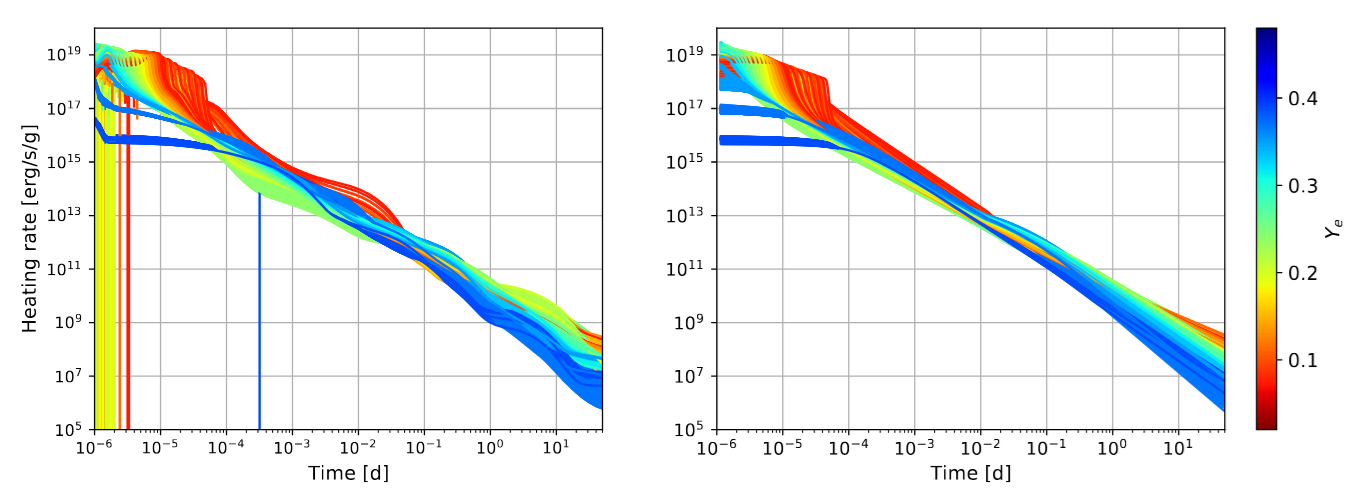
\includegraphics[width=1\linewidth]{../fig/fits.png}
\end{tcolorbox}


\end{column}

% Right column
\begin{column}{0.5\textwidth}
\vspace{-0.5cm}
\begin{tcolorbox}[
    colback=white,
    colframe=blue,
    colbacktitle=blue!50!black!50,
    title=Post-processing,
    fonttitle=\bfseries,
    rounded corners,
    boxrule=1pt,
    left=2mm, right=2mm, top=1mm, bottom=1mm
]
\begin{itemize}
   \scriptsize  
    \item KNEC code for light curves
    \begin{itemize} 
	\scriptsize
	\item 	Magistrelli et al. 2025
    \end{itemize}
   \scriptsize
    \item WinNet for nucleosynthesis
    \begin{itemize}
	\scriptsize
	\item fed with backwards time integrated tracers
	\item enough tracers to resolve the total mass $\sim{4.2}\times10^{4}$
	\item Reichert et al. 2023
    \end{itemize}
\end{itemize}
 
\includegraphics[width=0.6\linewidth]{../fig/winnet_logo_light_theme.png}
\end{tcolorbox}

\end{column}


\end{columns}

\end{frame}


\begin{frame}{Elements distribution's dependence on $\phi$}
\begin{columns}

\column{0.6\textwidth}
\centering
% --- First row ---

\includegraphics[width=0.45\linewidth]{../fig/blh_vlr_hr_constatm/Masses_sections_phi.pdf}%
\hspace{0.04\linewidth}%

\includegraphics[width=0.45\linewidth]{../fig/sfho_vlr_hr_constatm/Masses_sections_phi.pdf}

\vspace{2mm}

% --- Second row ---

\includegraphics[width=0.45\linewidth]{../fig/dd2_135_vlr_hr_constatm/Masses_sections_phi.pdf}%
\hspace{0.04\linewidth}%

\includegraphics[width=0.45\linewidth]{../fig/dd2_180_vlr_hr_constatm/Masses_sections_phi.pdf}

\column{0.4\textwidth}
\scriptsize
\begin{itemize}
	\item SFHo\_q1.0 and DD2\_q1.0 show stronger $\phi$ dependence for elements above $A\sim134$
	\item SFHo\_q1.0 and DD2\_q1.0 production varies by less than a factor $\lesssim 2$
	\item Largest variations for BLh\_q1.43 and DD2\_q1.67 occur for $A \gtrsim 134$
	\item Variations can reach factors of $\sim 5$--$10$
\end{itemize}

\end{columns}
\end{frame}

%------------------------------------------------
\begin{frame}{Lanthanides and Actinides DD2\_q1.67}

\begin{columns}[t] % top-aligned

% ----- Left image -----
\column{0.5\textwidth}
	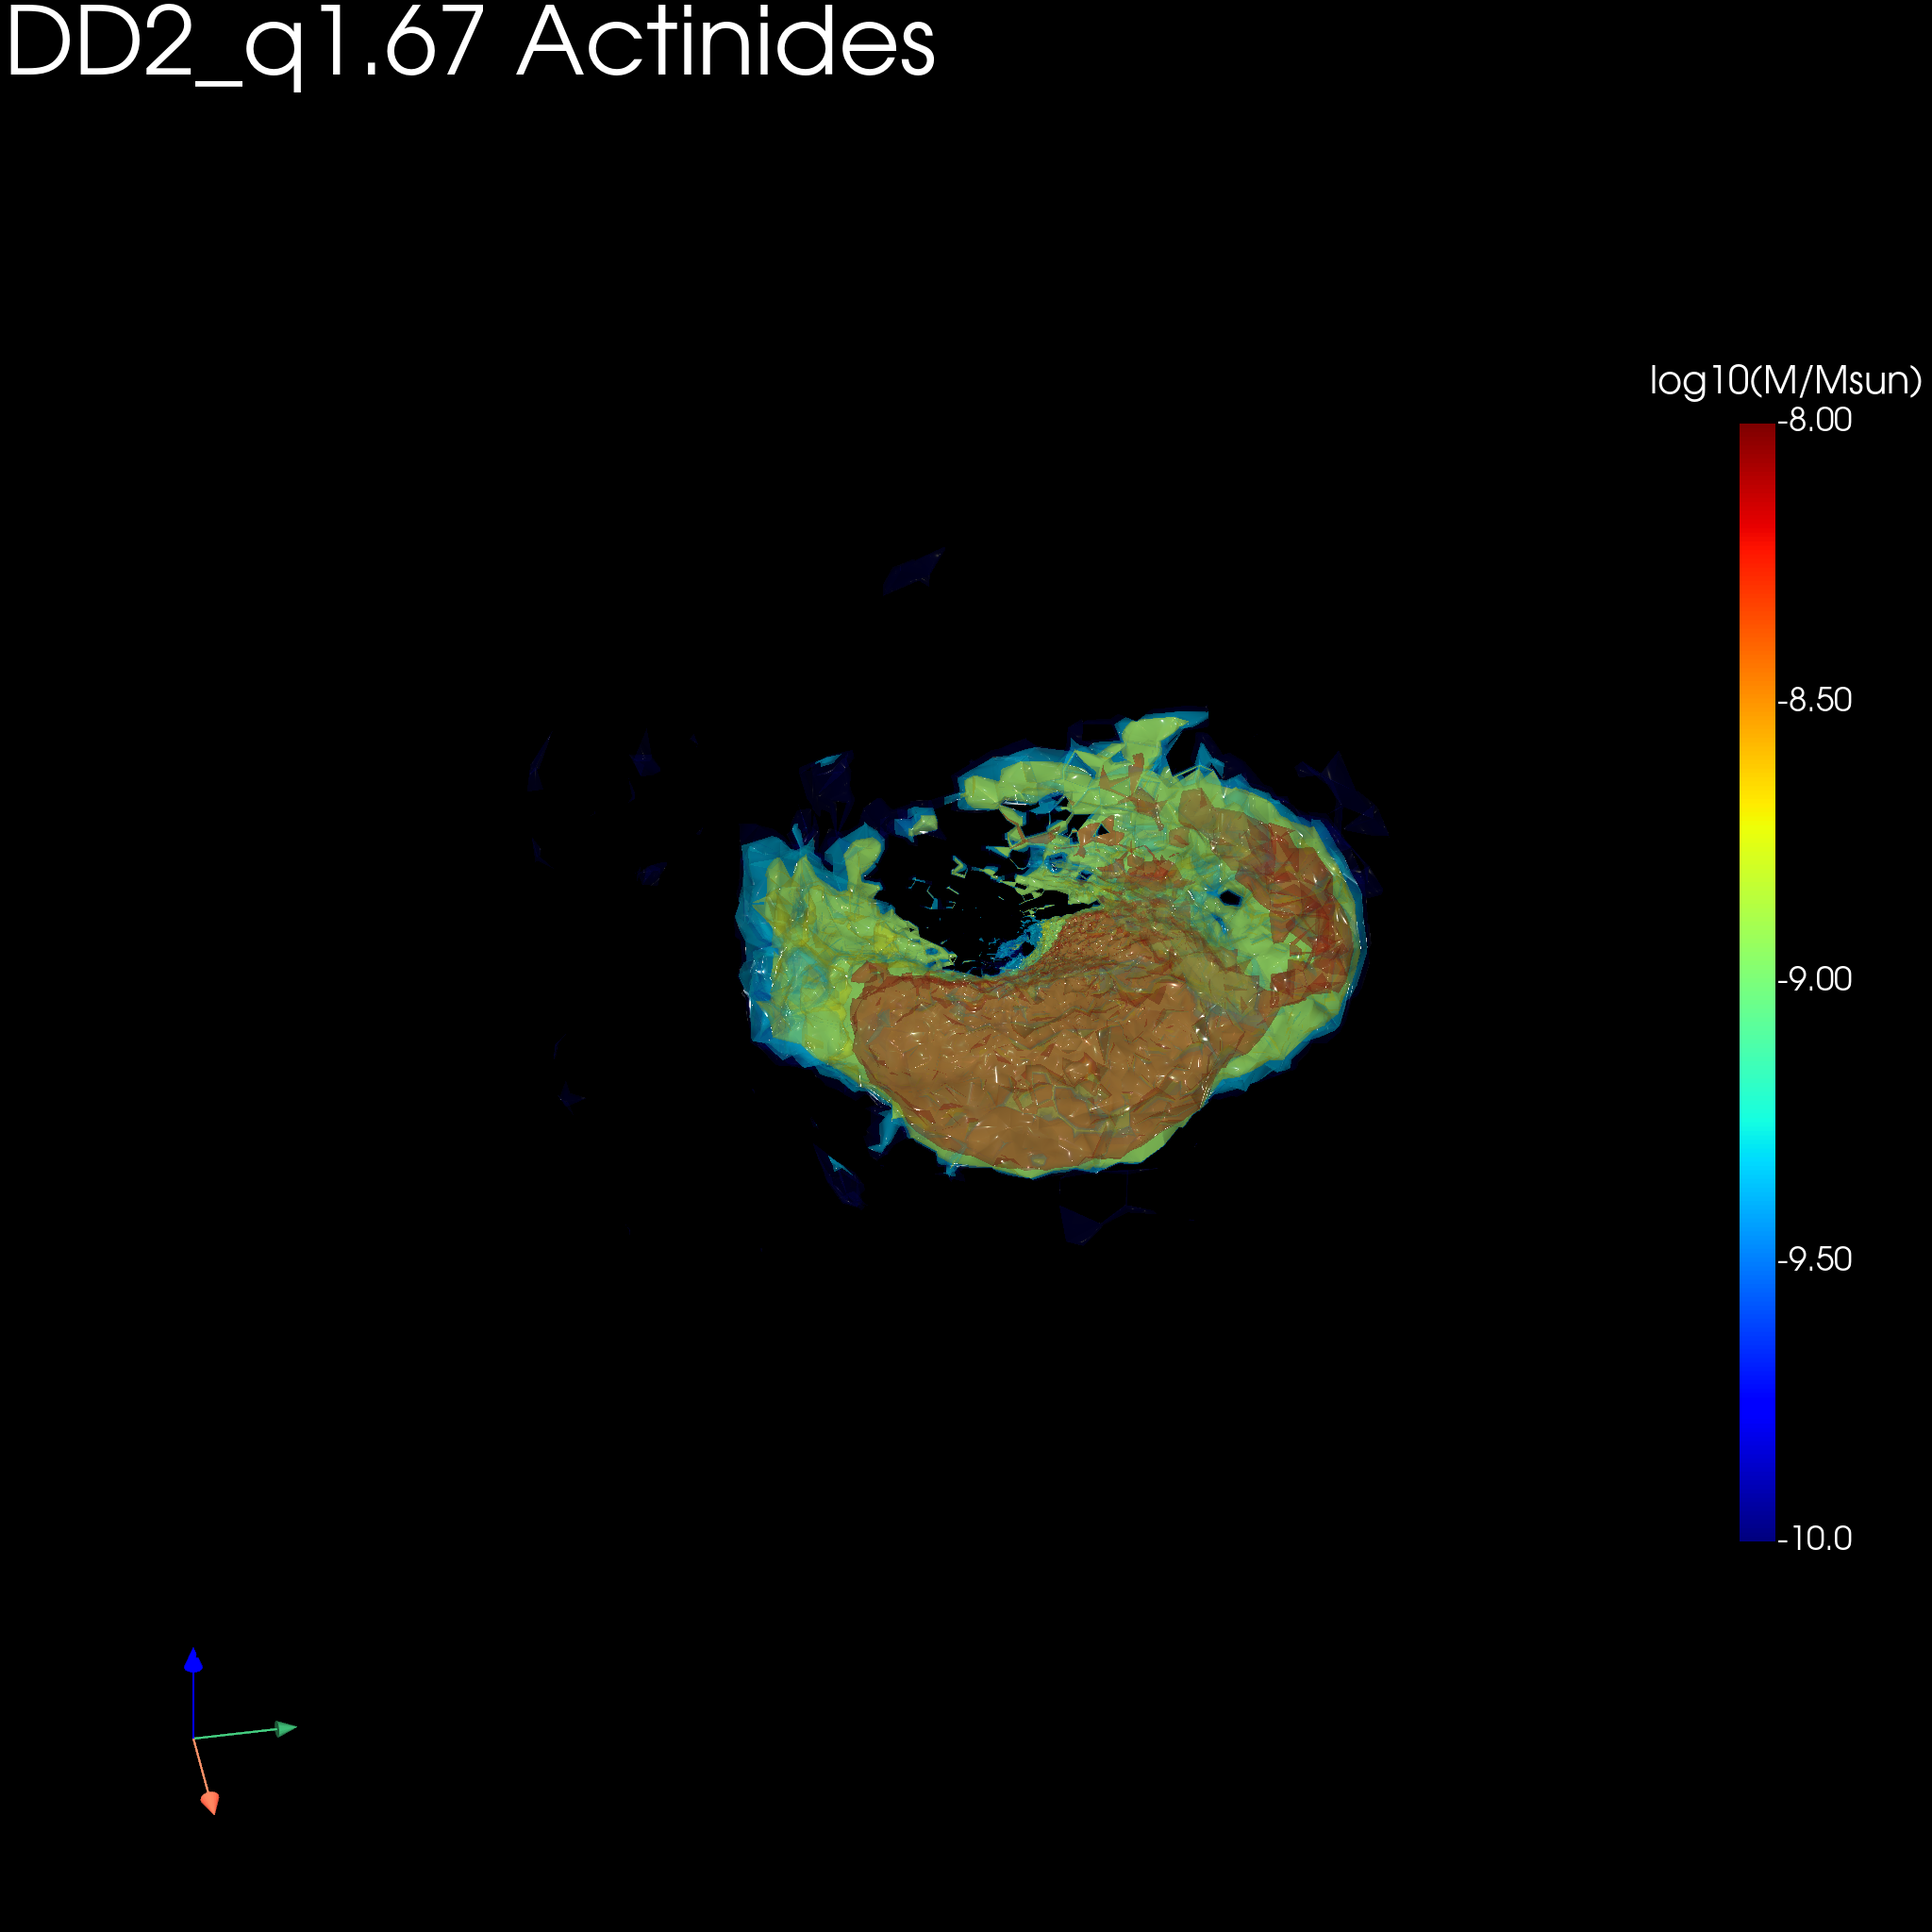
\includegraphics[width=\linewidth]{../fig/dd2_180_vlr_hr_constatm/DD2_q1.67_Actinides_frame_100.png}

% ----- Right image -----
\column{0.5\textwidth}
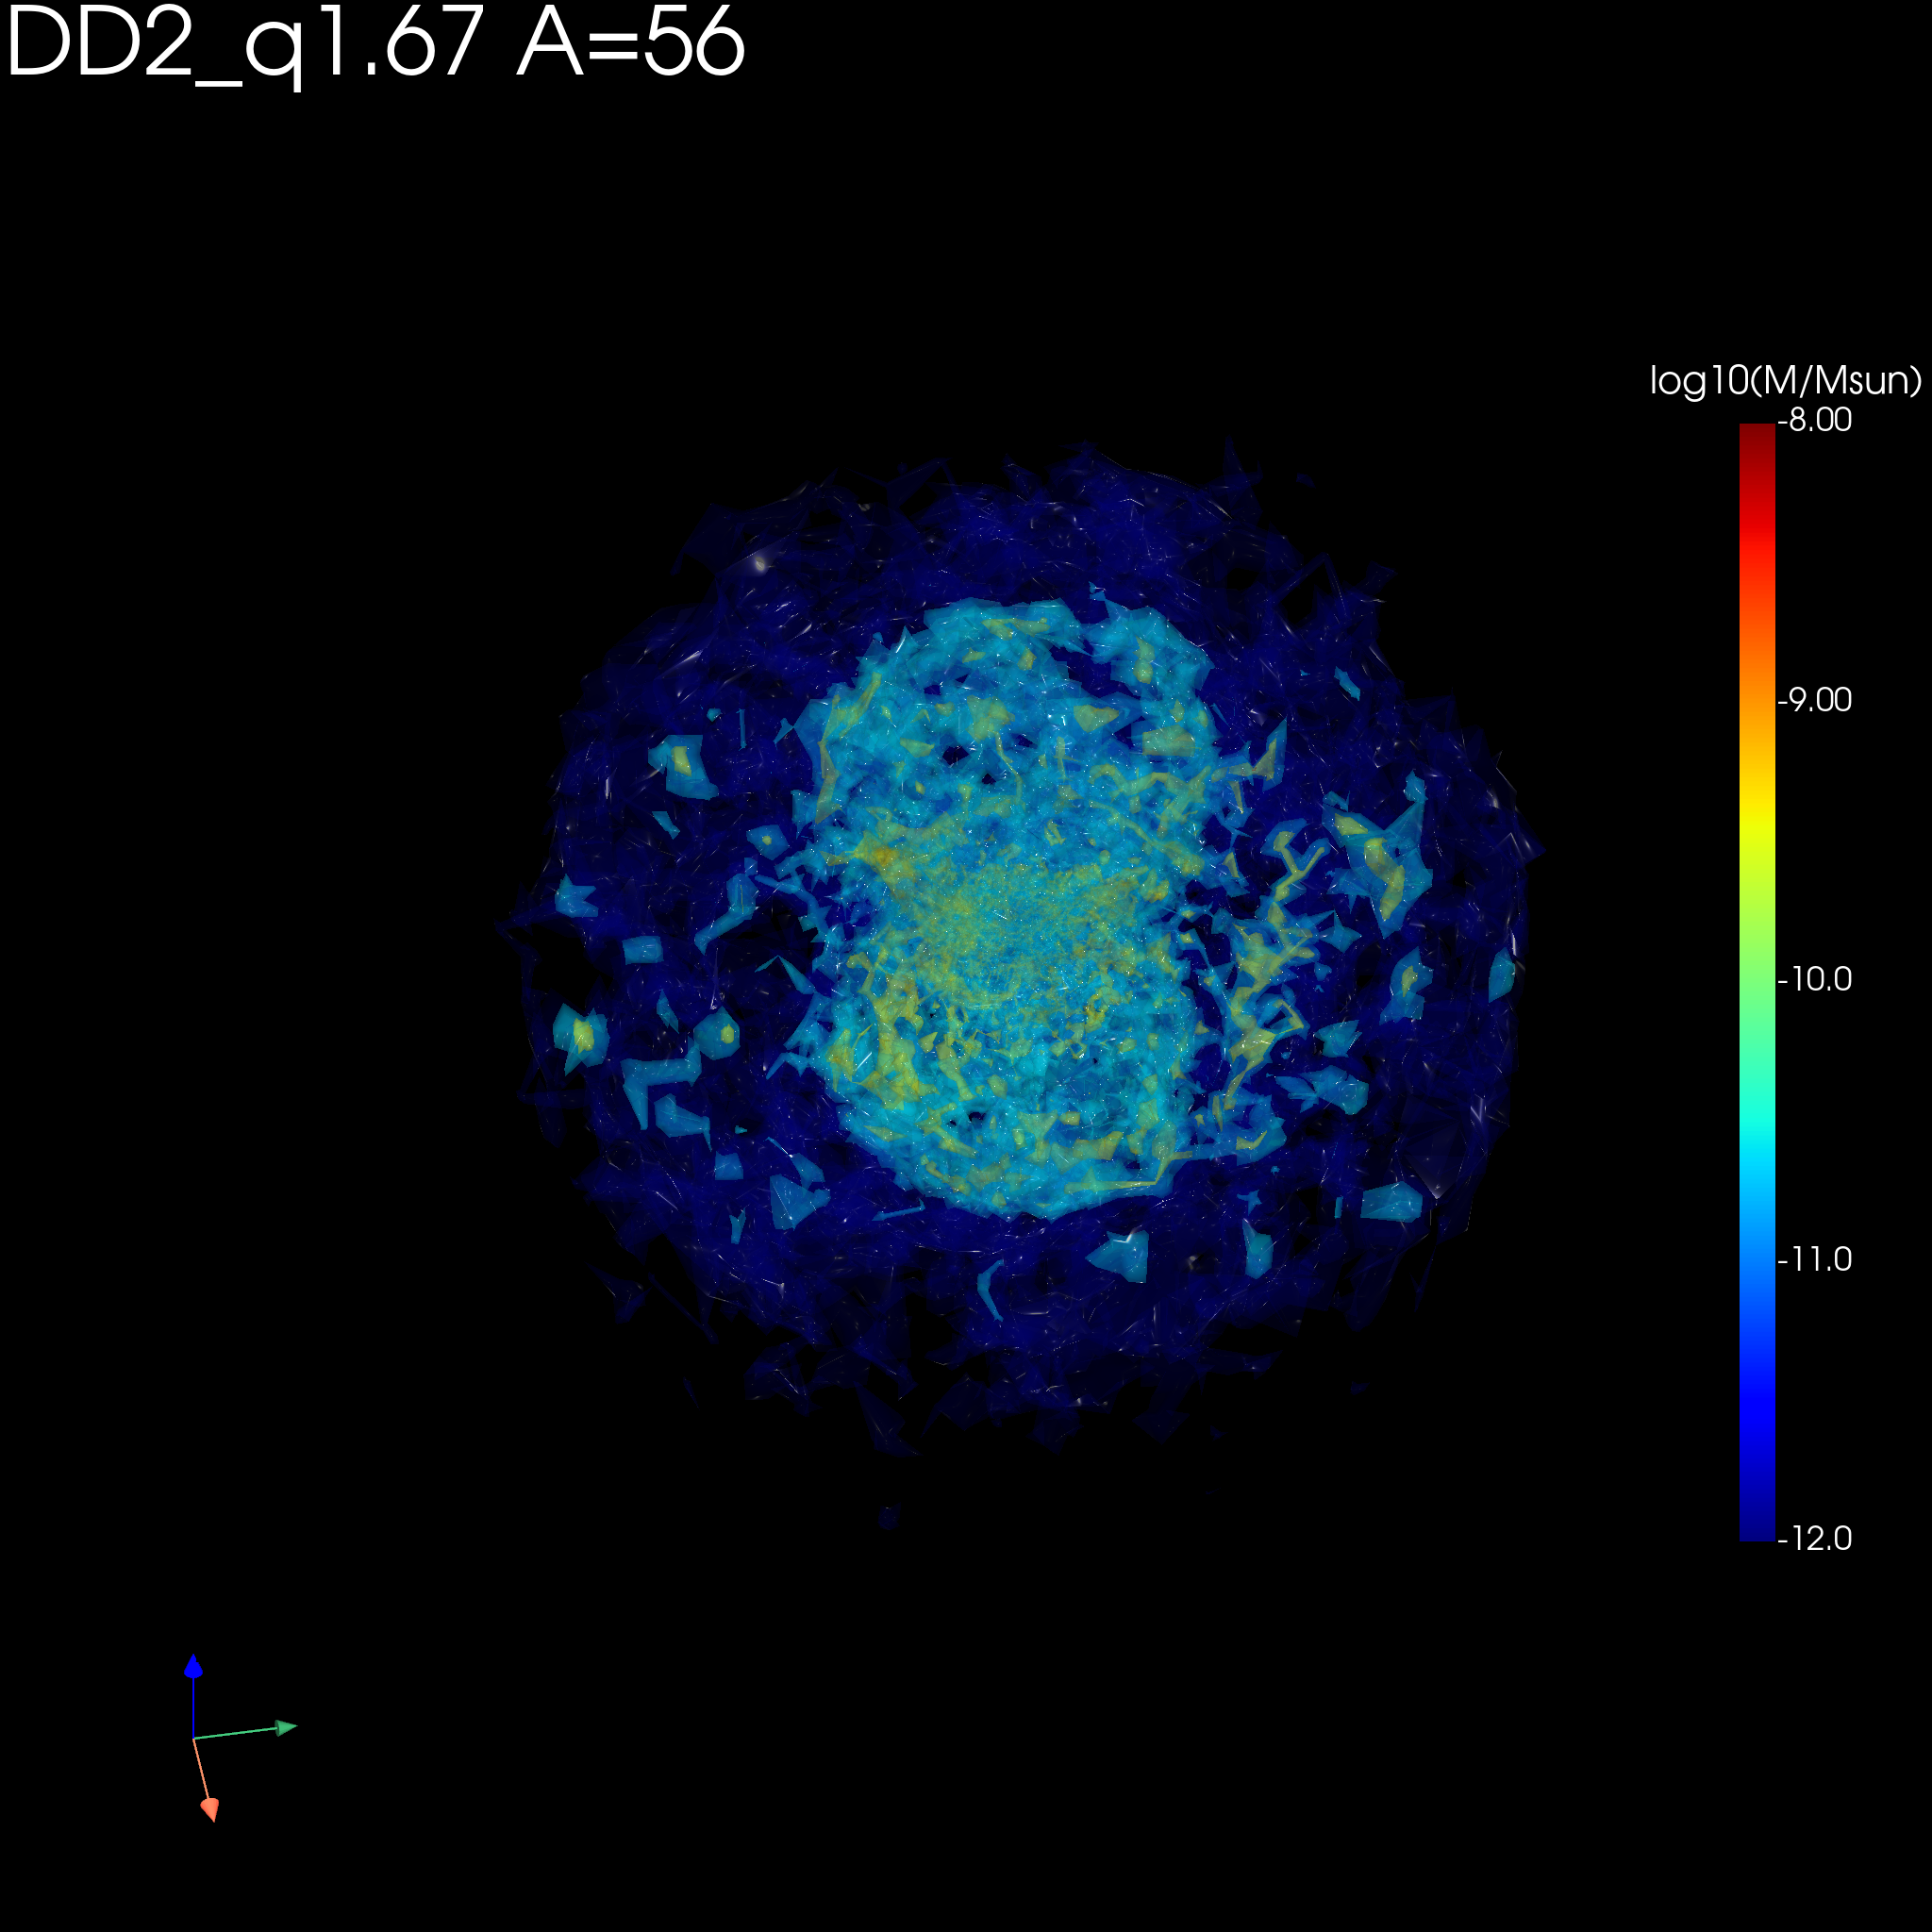
\includegraphics[width=\linewidth]{../fig/dd2_180_vlr_hr_constatm/DD2_q1.67_A=56_frame_100.png}

\end{columns}

\end{frame}



\begin{frame}{Dynamics}

\begin{columns}[t]

% ----- Left column -----
\column{0.5\textwidth}
\centering

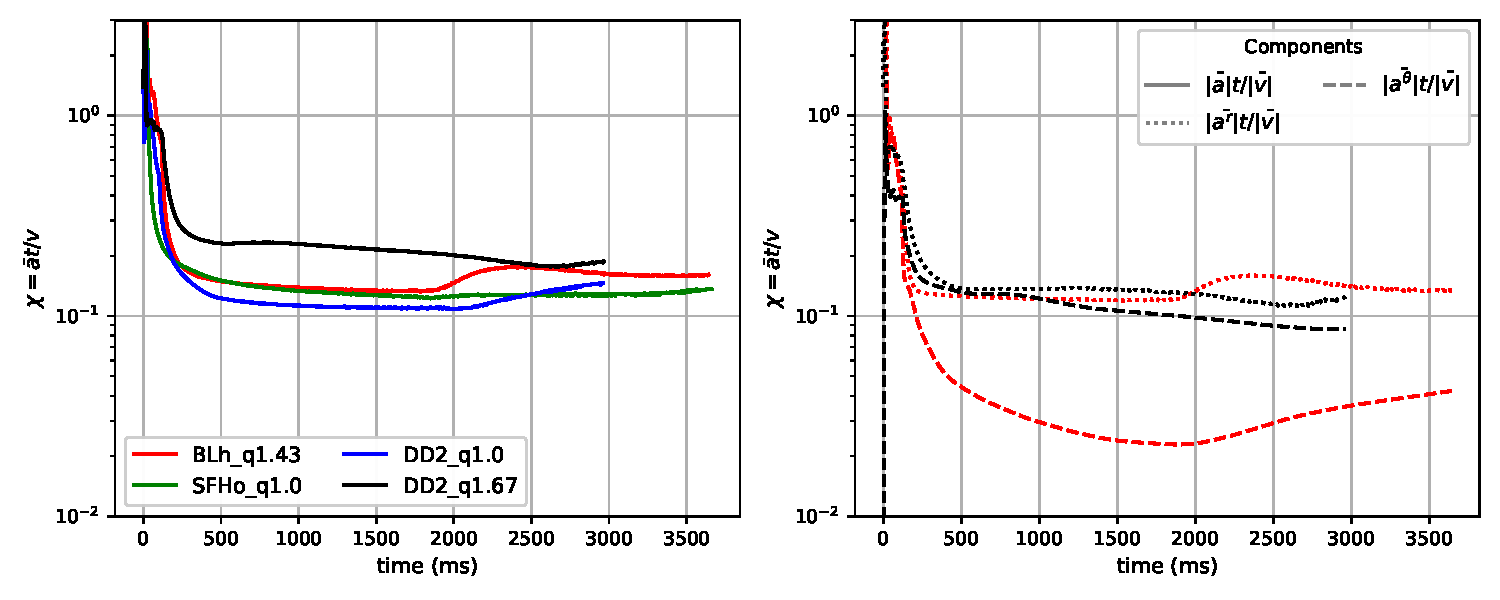
\includegraphics[width=\linewidth]{../fig/model_comparison/Chi_joined.pdf}

\vspace{-0.3em}

\hspace{0.15\linewidth}%

\includegraphics[width=0.7\linewidth]{../fig/model_comparison/Expansion_and_heating_energies_v3.pdf}

% ----- Right column -----
\column{0.5\textwidth}

\begin{itemize}\scriptsize
    \item $\chi \equiv \bar{a} t / v$
    \item All models show decaying $\chi$ after the end of injection
    \item Models show increasing $\chi$ at $t \sim 2\,\mathrm{s}$
    \begin{itemize}\scriptsize
        \item Due to mass exiting the grid
    \end{itemize}
    \item DD2\_q1.67 has significant non-radial motion
    \begin{itemize}\scriptsize
        \item Due to elevated nuclear heating
    \end{itemize}
\end{itemize}

\vspace{0.5em}

\centering
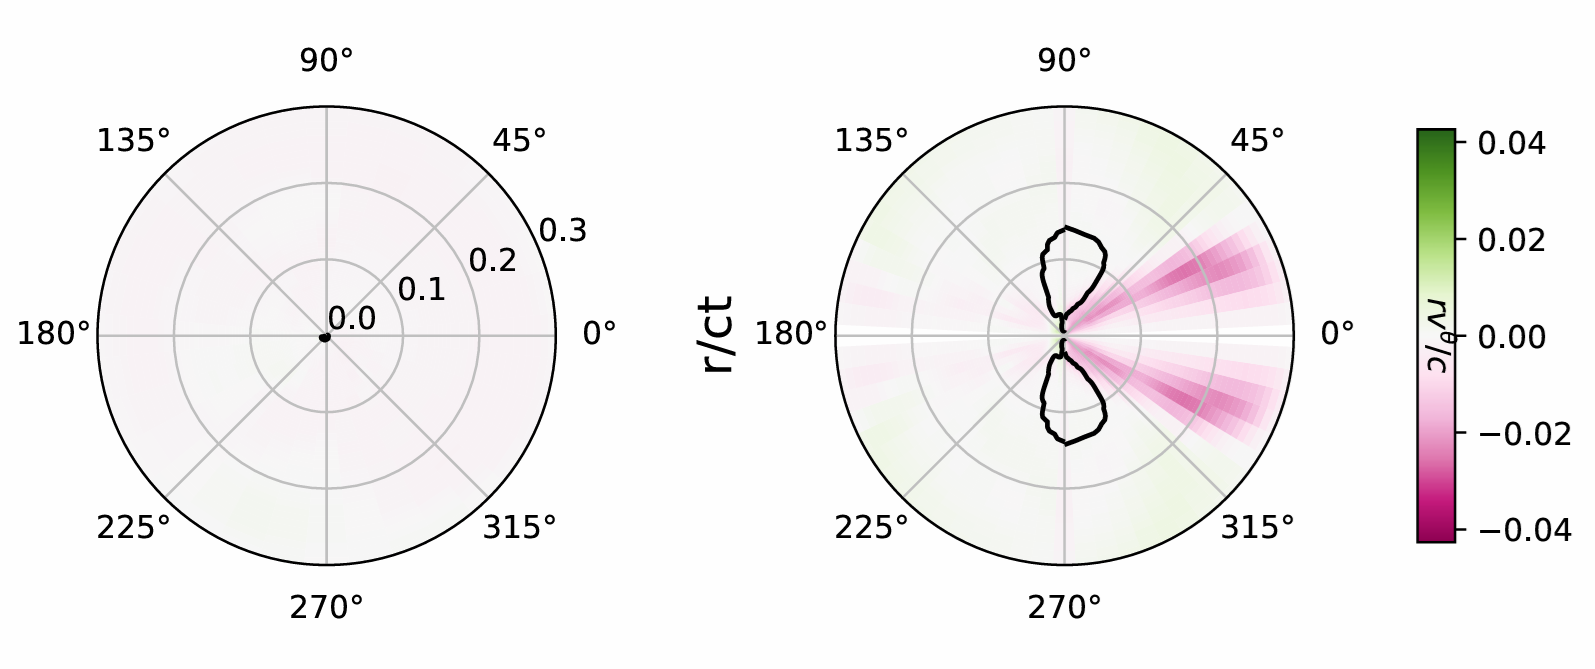
\includegraphics[width=\linewidth]{../fig/dd2_180_vlr_hr_constatm/velocities_final_cropped.png}

\end{columns}
\end{frame}


\begin{frame}{Methods (Developments - MHD)}
\begin{columns}

% Left column
\begin{column}{0.5\textwidth}
\begin{tcolorbox}[
    colback=white,
    colframe=blue,
    colbacktitle=blue!50!black!50,
    title=GRMHD simulations,
    fonttitle=\bfseries,
    rounded corners,
    boxrule=1pt,
    left=2mm, right=2mm, top=1mm, bottom=1mm
]
\begin{itemize}   
   \scriptsize
    \item Original THC Simulations full GRhydro + M1 (Radice \& Benuzzi 2023, Benuzzi et al. 2025; Gutierrez et al. 2024)
    \begin{itemize}
    	\item Athena++ extensions (Stone et al. 2020)
    	\item Superimpose $\vec{B}$-fields
   \end{itemize}
    \item Original AthenaK Simulations full GRMHD + M1 
    \begin{itemize}
    	\item Athena++ extensions (Stone et al. 2020)
    	\item With $\vec{B}$-fields data
   \end{itemize}

\end{itemize}

\end{tcolorbox}


\end{column}

% Right column
\begin{column}{0.5\textwidth}
\vspace{-0.5cm}
\begin{tcolorbox}[
    colback=white,
    colframe=blue,
    colbacktitle=blue!50!black!50,
    title=$\vec{B}$ injection,
    fonttitle=\bfseries,
    rounded corners,`
    boxrule=1pt,
    left=2mm, right=2mm, top=1mm, bottom=1mm
]

\begin{itemize}
\item What $\vec{B}$ field to superimpose ?
 	\begin{itemize}
	\item $ \vec{B} = \vec{B}_{pol}(1+\psi(r,\theta,\phi,t ,\vec{k})) + \vec{B}_{tor}(\delta(r,t, \vec{l}))$
	\item $\vec{k}$ and $\vec{l}$  are random wave lengths coefficients  
	\item More motivated randomization?
	\end{itemize}
\item Simulated $\vec{B}$-fields ?
 	\begin{itemize}
	\item Wave lengths of $\vec{B}$ may need to match new grid
	\item Cartesian $\rightarrow$ Spherical grids matching
 	\end{itemize}

\end{itemize}   


\end{tcolorbox}

\end{column}

\end{columns}

\end{frame}


\begin{frame}{Accretion Induced Collapse (of White Dwarf)}

\begin{minipage}[t]{0.48\textwidth}
\vspace{0pt}
        \begin{figure}
                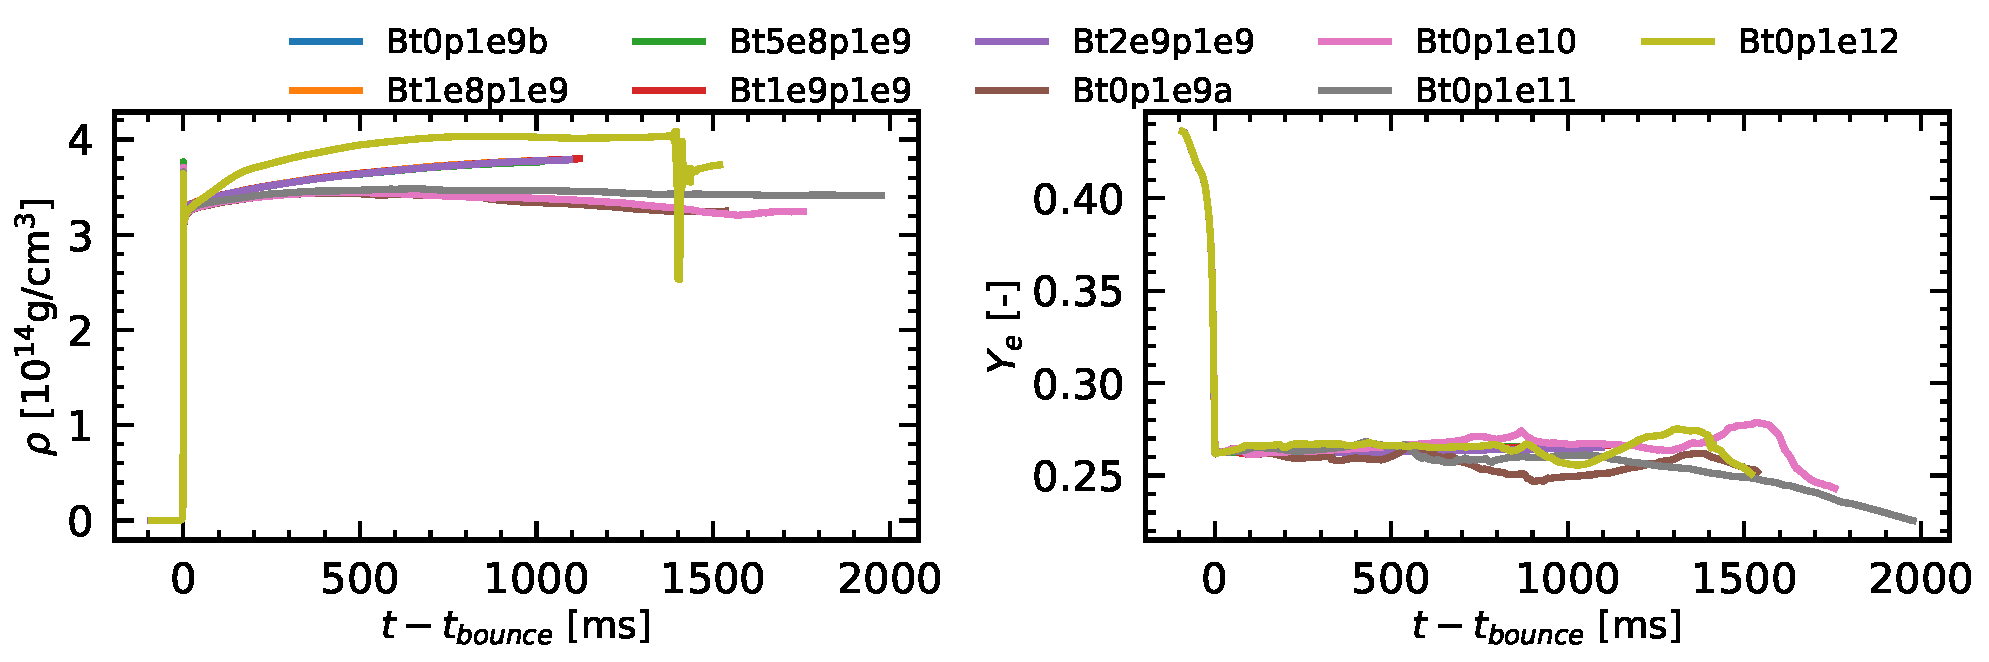
\includegraphics[width=1.1\linewidth]{../fig/AIC/Central_density_and_ye.pdf}
	      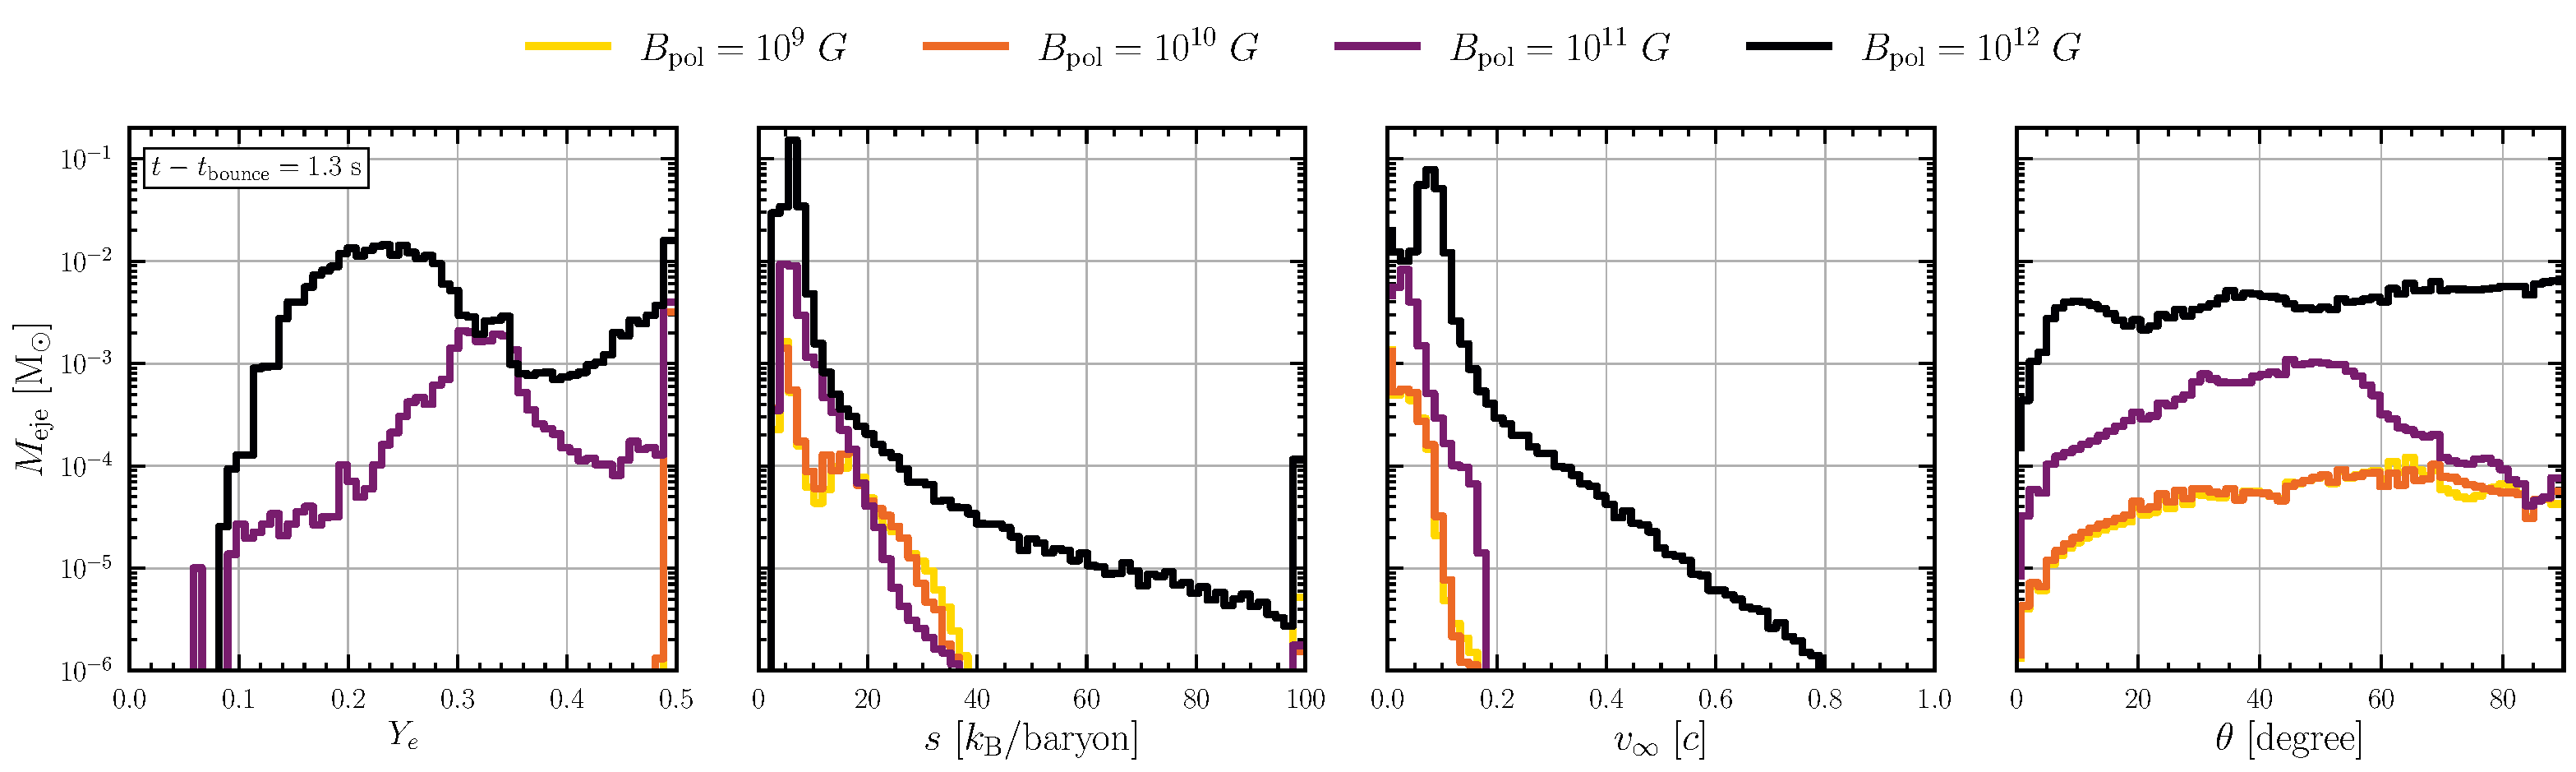
\includegraphics[width=1.1\linewidth]{../fig/AIC/fig_eje_histogram.pdf}
        \end{figure}

\end{minipage}
\hfill
\begin{minipage}[t]{0.45\textwidth}
\vspace{0pt}
\begin{tcolorbox}[
    colback=white,
    colframe=blue,
    colbacktitle=blue!50!black!50,
    title=Overview,
    fonttitle=\bfseries,
    rounded corners,
    boxrule=1pt,
    left=2mm, right=2mm, top=1mm, bottom=1mm
]
\begin{itemize}
   \scriptsize 
    \item WD with accretion history
    \item  $M\rightarrow  1.44 (1+\epsilon) M_{\odot}$ 
    \item  $Y_{e}\rightarrow Y_{e}(\rho)$ (until collapse) 
    \item M1 after collapse
    \item  MMA  (see 2306.04711)
    \item  LGRB + KN (see 2410.10938)
    \item magnetar formation (in prep.)
    \item Limitation: Isolated WD simulations (likely not true)

	
\end{itemize}
\end{tcolorbox}
\end{minipage}

\end{frame}


\begin{frame}{Questions}

\begin{minipage}[t]{0.48\textwidth}
\vspace{0pt}
        \begin{figure}
                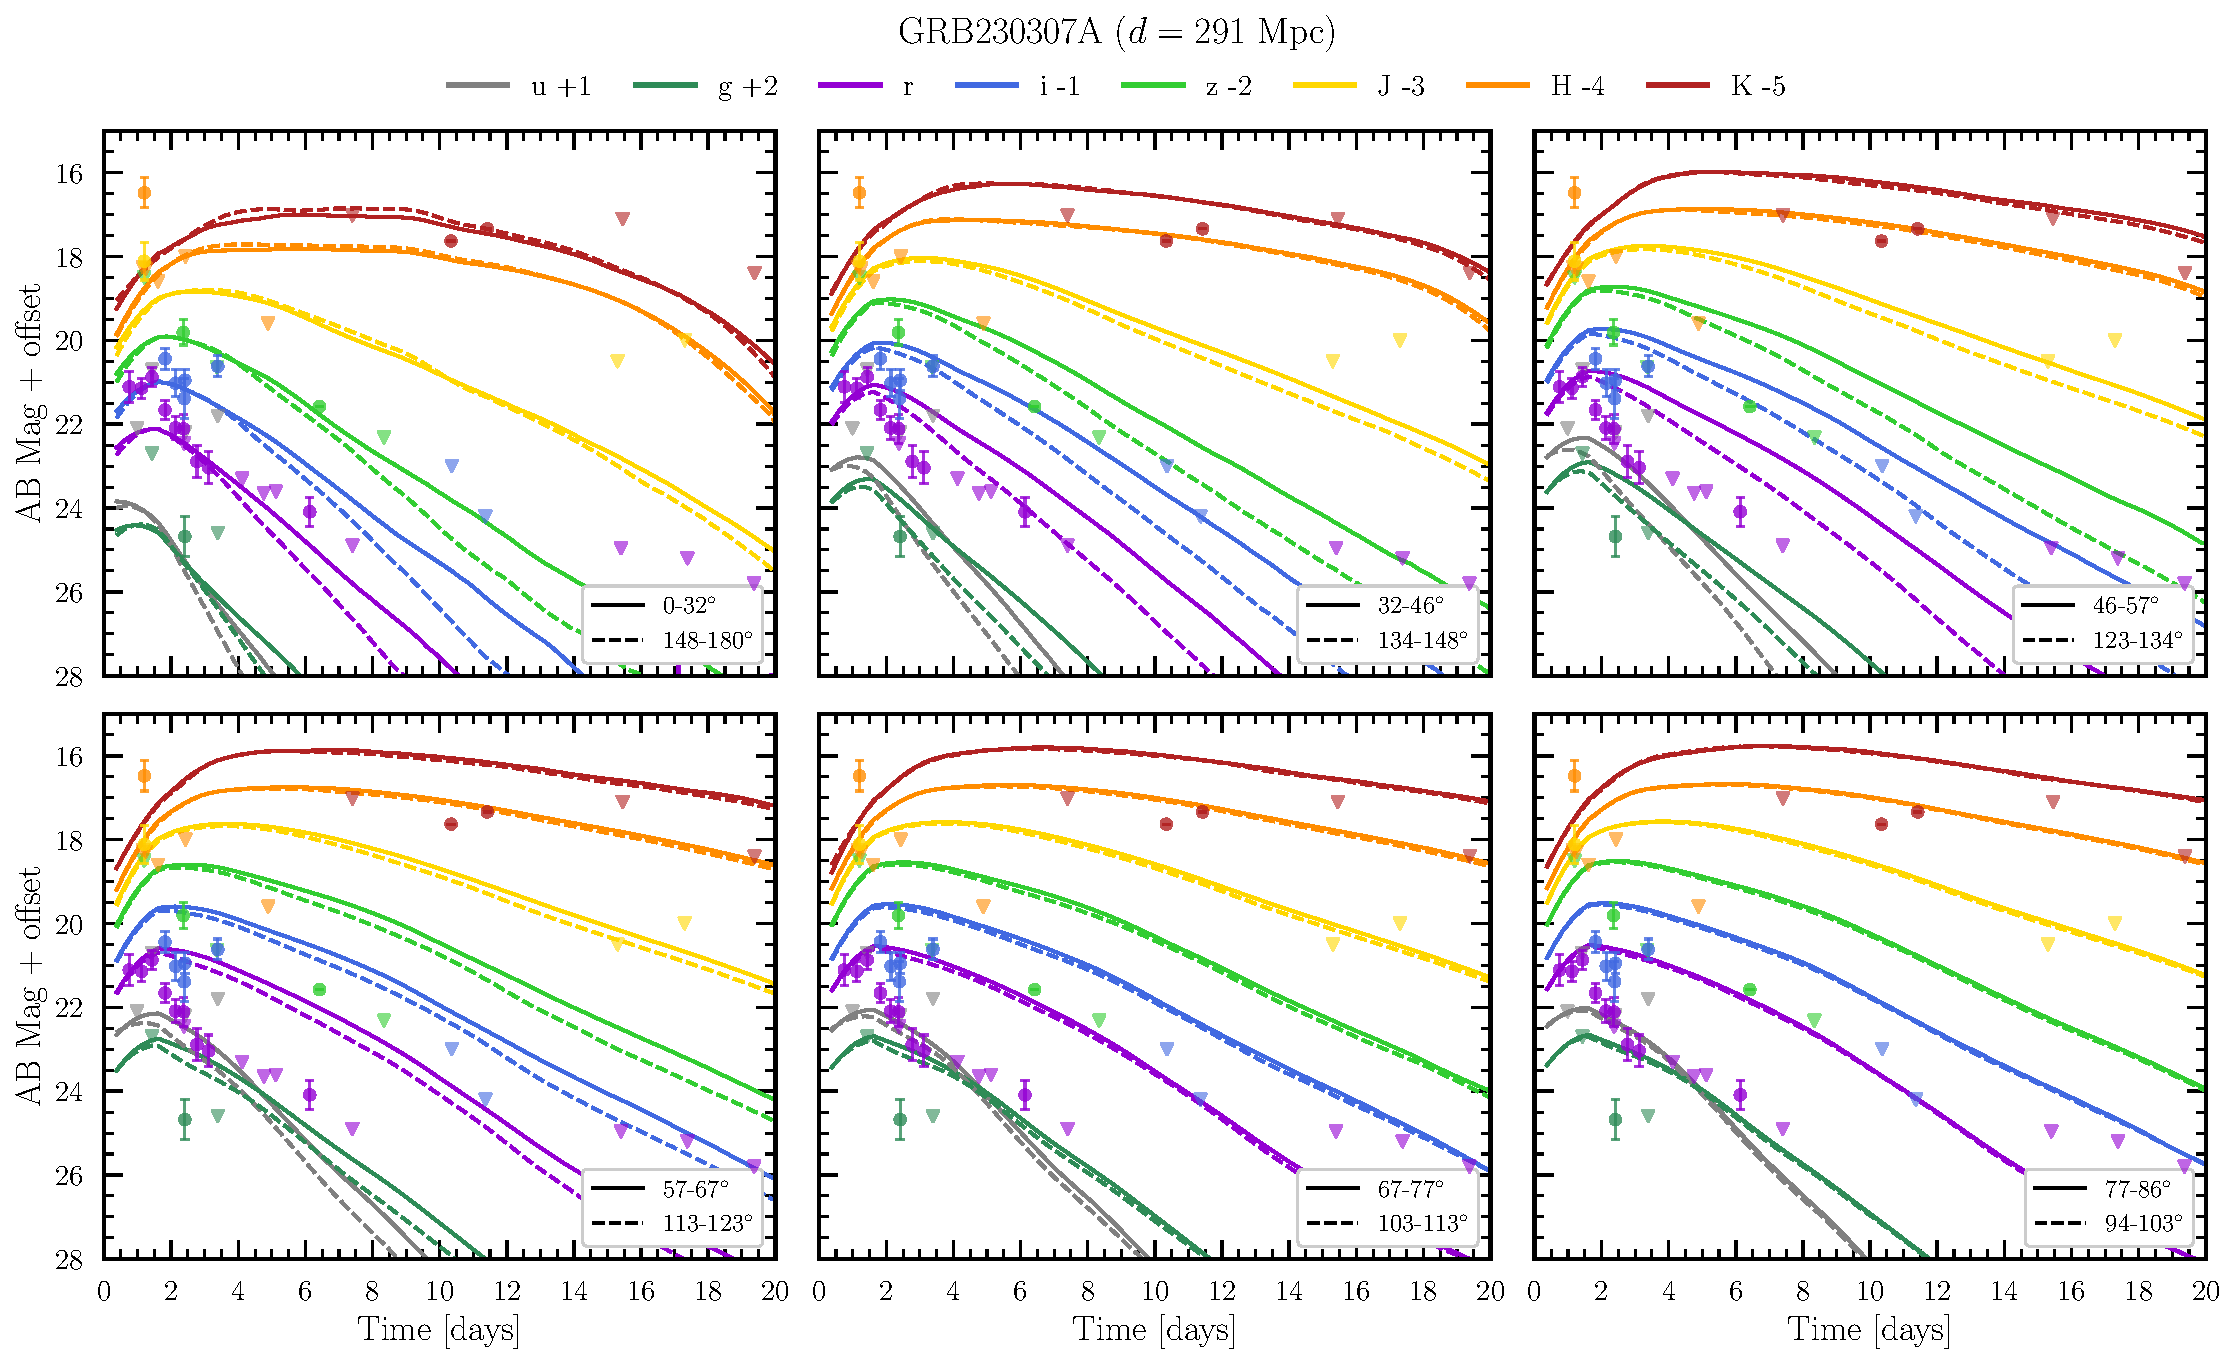
\includegraphics[width=1.1\linewidth]{../fig/AIC/H.pdf}

        \end{figure}

\end{minipage}
\hfill
\begin{minipage}[t]{0.45\textwidth}
\vspace{0pt}
\begin{tcolorbox}[
    colback=white,
    colframe=blue,
    colbacktitle=blue!50!black!50,
    title=Overview,
    fonttitle=\bfseries,
    rounded corners,
    boxrule=1pt,
    left=2mm, right=2mm, top=1mm, bottom=1mm
]
\begin{itemize}
   \scriptsize 
    \item WD with accretion history - Companion or disk
    \item WD may not accreate all mass before collapse
    \item Evolve ejecta of AIC with remans of companion
    \item Imprint on light curve or nucleosynthesis?
    \item Does it affect the aggreement foun with LGRB ? (see 2602.21291)
   \item Composition, mass, and distribution of the remains ?
	
\end{itemize}
\end{tcolorbox}
\end{minipage}

\end{frame}







\end{document}
